\begin{document}

% self defined colors for colored code (can add more colors)
\definecolor{green}{rgb}{0.1,0.5,0.2} % rgb defined between 0 and 1
\definecolor{blue}{rgb}{0,0.3,0.7}
\definecolor{purple}{rgb}{0.7,0,0.7}
\definecolor{gray}{rgb}{0.5,0.5,0.5}
\definecolor{codeorange}{rgb}{0.9,0.3,0}

% writing code in the document as list
% can be changed, add changed version before your code (possible to have multiple versions within one doc)
\lstset{ 
  basicstyle=\ttfamily\UseRawInputEncoding\small,
  extendedchars=true, % lets you use non-ASCII characters; for 8-bits encodings only, does not work with UTF-8
  breaklines=true,                 
  escapeinside={\%*}{*)}, % if you want to add LaTeX within your code
  keepspaces=true,
  morekeywords={*,...}, % if you want to add more keywords
  showstringspaces=false,          
  tabsize=2, % sets default tabsize to 2 spaces
  numbersep=5pt, % how far the line-numbers are from the code
  numbers=left,                   
  numberstyle=\tiny\color{gray},
  stringstyle=\color{purple},
  commentstyle=\color{gray},
  keywordstyle=\color{blue},
  identifierstyle=\color{codeorange}
}

%=================================================================
%                           Start Document
%=================================================================
\setstretch{1.6}

\section{Results}
\lhead{Results} % section header

\subsection{Open Loop Stimulation Sequence}
The four muscle open loop stimulation sequence laid out in the methods section on open loop stimulation, was tested on three healthy subjects between the ages of 22 and 25, two female and one male. This was done before moving further with closed loop development, to ensure that the stimuation sequence was generalizable across individuals. During the setup phase the optimal placements for the electrodes for each individual subject were found along with the motor threshold and the maximum tolerable intensity. The stimulation intensity was set as the value in which the functional movement associated with that muscle was achieved and the movement resembled the reference videos mentioned in the methods section as closely as possible.

The subjects were then fitted with the Xsens Awida  motion capture system IMUs. The Xsens Awinda is a wireless, wearable system that uses IMUs specifically designed to capture human movement without the need for cameras or external markers \cite{noauthor_mvn_nodate}. It is often used for validation in literate since it provides accurate, portable motion tracking. The system was calibrated before subjects were instructed to go on the treadmill. 

\todo{XSens figure}

The treadmill was set to 1.5km/h and subjects were instructed to relax as much as possible the muscles in the leg which would be stimulated. The stimulation ran for 3 minutes and thereafter a baseline measurement was done in which the subjects muscles were not stimulated and they simply walked on the treadmill for three minutes. 

To analyze the results of the stimulation experiment, data from the MVNX files produced by the Xsens system were processed in Python to extract and compare the knee angles across gait cycles with and without stimulation. The Xsens system includes inbuilt sensor fusion capable of outputting the knee angle this was then loaded for processing by using the \texttt{load\_mvnx} library. 

To align and normalize the gait cycles, the peaks in the knee flexion data were identified using the \texttt{scipy.signal} module. Consecutive peaks were used to segment the flexion data into individual gait cycles. To ensure meaningful averaging across cycles, the segmented gait cycles were normalized in length. Each cycle was interpolated to 100 equidistant points, corresponding to a percentage of the gait cycle. Once normalized the gait cycles were averaged point by point to compute the mean knee angle and standard deviation. The data was then shifted so that the peak would be centered at the 75\% mark. The standard deviation values were used to create the upper an lower bounds of the colored regions around the mean which is plotted as a continuous curve. 

\begin{figure}[h]
    \centering
    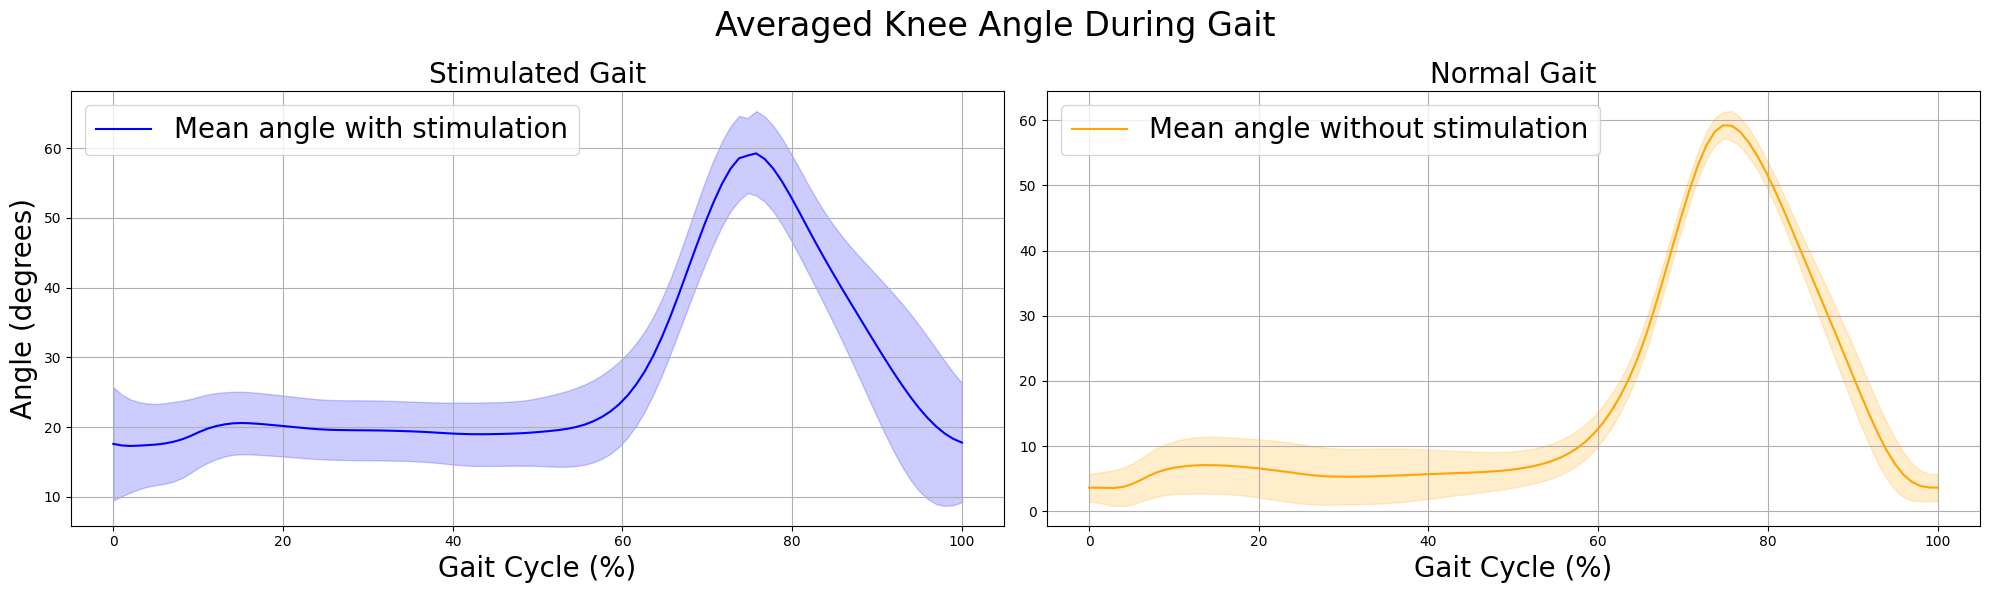
\includegraphics[width=0.99\linewidth]{images/alexisoutput1.png}
    \caption{Caption}
    \label{fig:alexisout}
\end{figure}

\begin{figure}[h]
    \centering
    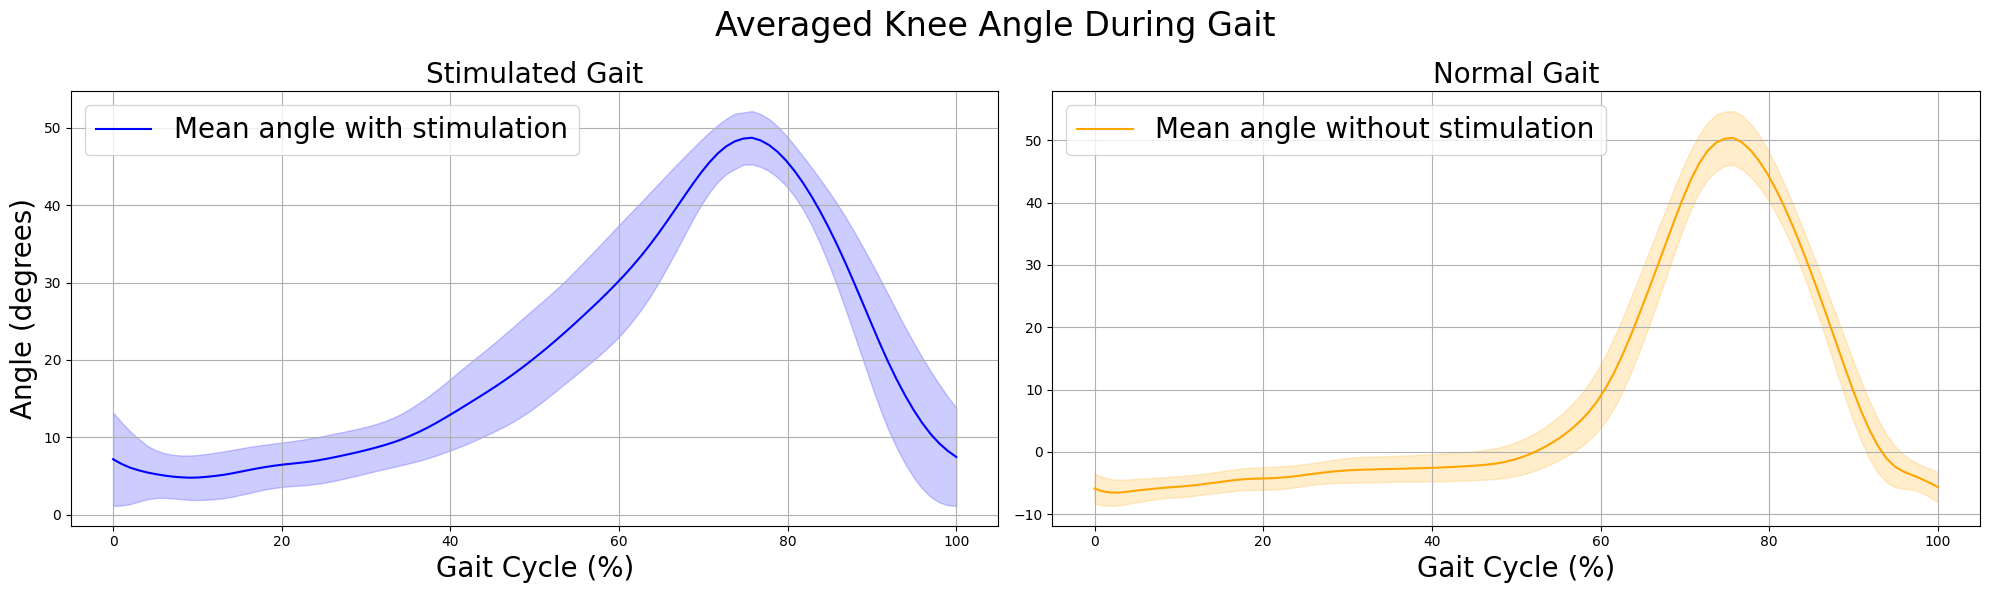
\includegraphics[width=0.99\linewidth]{images/katlaoutput1.png}
    \caption{Caption}
    \label{fig:katlaout}
\end{figure}

\begin{figure} [h]
    \centering
    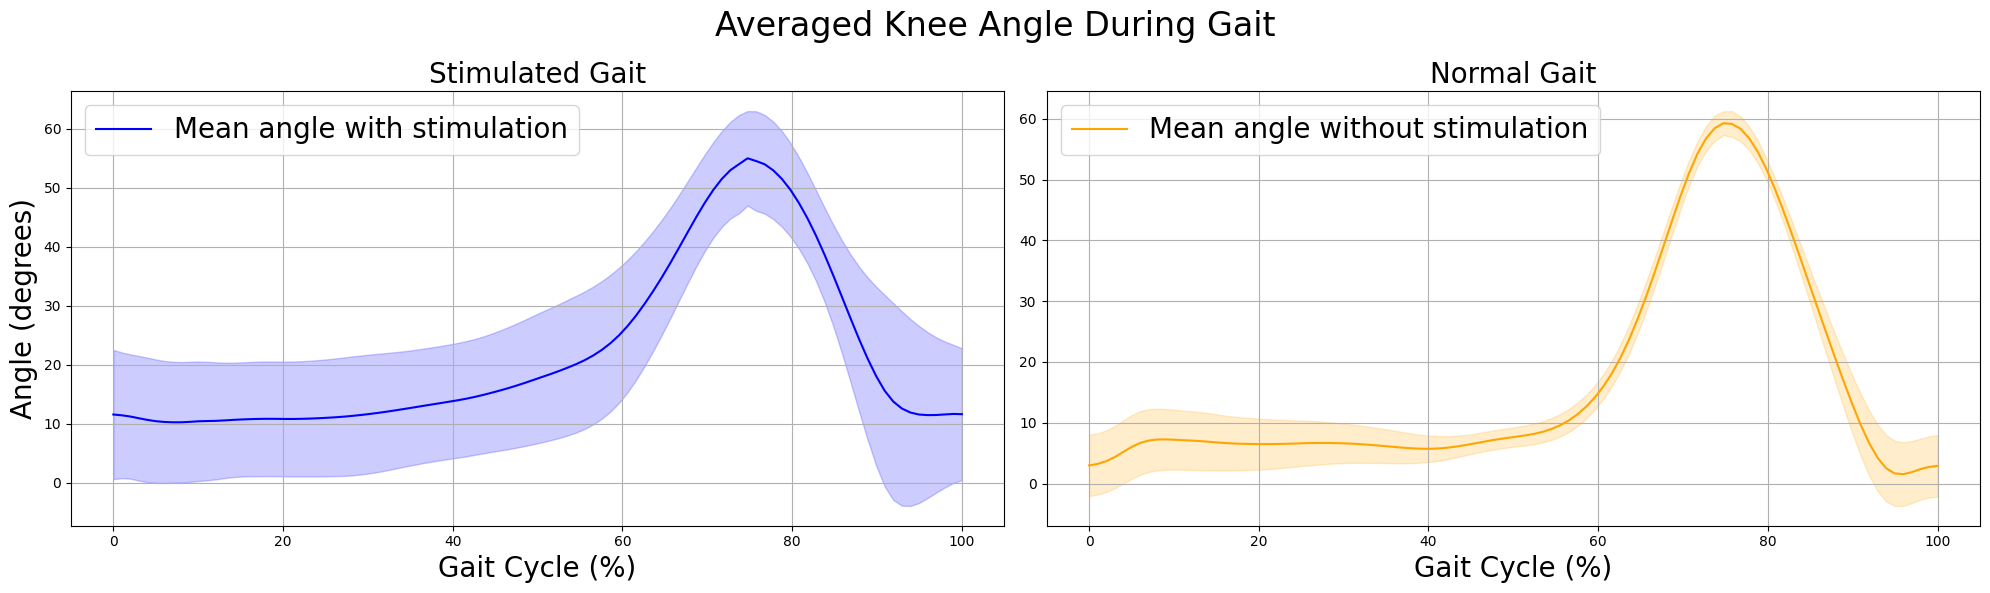
\includegraphics[width=0.99\linewidth]{images/leonioutput1.png}
    \caption{Caption}
    \label{fig:leoniout}
\end{figure}

The results from the three subjects can be seen in figure \ref{fig:alexisout}, \ref{fig:katlaout} and \ref{fig:leoniout}. A observation across all subjects is that the shapes of the mean knee angle curves are remarkably similar between the stimulated and non-stimulated conditions. This is despite natural differences in the gait patterns of the individuals. This similarity indicates that the general kinematic pattern is preserved under electrical stimulation. However, the standard deviation around is noticeably larger in the stimulated condition for all subject. Indicating increased variability in the step during stimulated walking.

One observed challenge during open-loop stimualtion was that, in some instances, subjects took disproportionately small or large steps with the contralateral (non-stimulated) leg. This disrupted the gait rhythm and caused the walking pattern to fall out of sync with the stimulation pattern. Leading to unstability until the subjects gait was again syncronized with the stimulation. This issue was particularly evident in subject 3 (figure \ref{fig:leoniout}), which resulted in the especially large standard deviation. This issue reflects the lack of adaptability when using an open-loop stimulation system, which does not account for real-time changes in the subject's gait rhythm or step length. 

However, overall, the results show that the open loop stimulation sequence is generalizable and works across individuals, meaning that the project could move on to further develop the closed-loop which bases its stimulation sequence on this result.


\subsection{Knee Angle Estimation}
Accurate knee angle estimation is critical for the closed loop FES application. Therefore the Madgwick knee angle stimation technique was validated by comparing the IN-House IMU based knee angle estimation with the DELSYS IMU base knee angle estimate as a benchmark. Delsys IMUs provide high-quality orientation data by leveraging advanced sensor fusion algorithms, designed specifically for biomechanical and movement studies \todo{source add more detail}. 

\begin{wrapfigure}{r}{}
    \centering
    \includegraphics[width=0.5\linewidth]{}
    \caption{Caption}
    \label{fig:enter-label}
\end{wrapfigure}

The method for knee angle estimation using the In-House IMUs is described throroughly in the methdods section "Knee Angle Estimation". The method for extracting the knee angle from the Delsys sensors involved capturing the orientation data that the sensors provide already having used sensor fusion. The relative orientation between the two sensors is then computed by taking the inverse of the thighs sensoræs rotation and applying it to the shank sensoræs rotation. This relative rotation is then converted to Euler angles from which the rotation about the x-axis is extracted:
\begin{equation}
    \theta_{\text{knee}} = \text{Euler}_x \left( \mathbf{q}_{\text{thigh}}^{-1} \otimes \mathbf{q}_{\text{shank}} \right)
\end{equation}

The validation experiment consisted of mounting the Delsys IMUs and In-House IMUs on the thigh and shank as seen in figure \todo{ref}. The subject was then instructed to sit and move their leg from resting on the ground at approximately a 90 degree angle to resting it on a chair at a full extension, meaning approximately zero degrees. In order to compare the two estimates, the computed knee angles were synchonized and compared over a shared time range. Linear interpolation was applied to both datasets to align them temporally, accounting for potential differences in sampling rates and starting times. The synchronized data allows for a direct comparison as can be seen in figure \ref{fig:t11}. 

\begin{figure} [H]
    \centering
    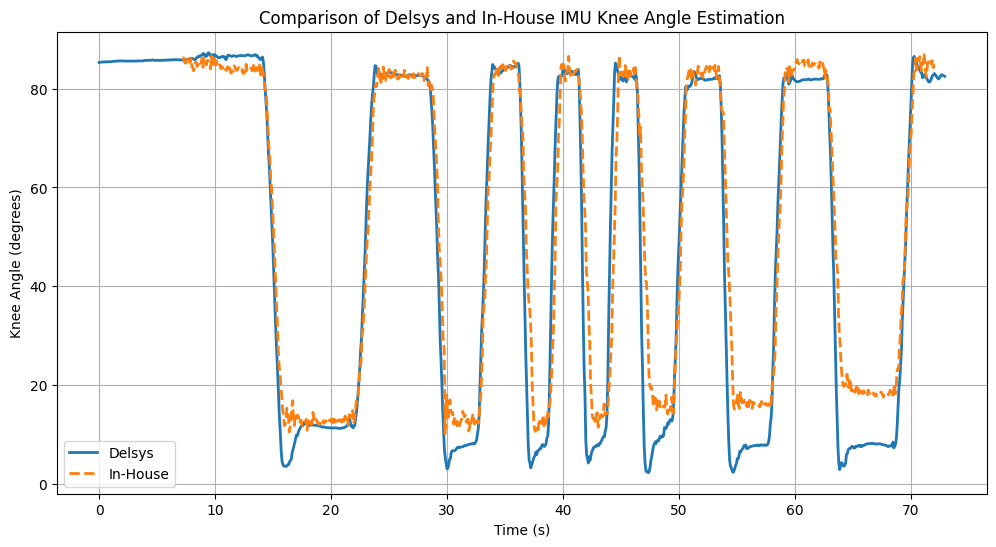
\includegraphics[width=0.95\linewidth]{images/T11_betterplotting.png}
    \caption{}
    \label{fig:t11}
\end{figure}

The results show that the adapted Madgwick filter does a good job of estimating the knee angle. However we see some slight drift, even though the Madgwick filter should in theory be robust to drift. It is however worth noting here that there are some clear inaccuracies in the Delys derived knee angle as well. Specifically we observe that there is a valley in the calculated knee angle followed by a flattening out of the curve when the knee is extended, this does not reflect the actual movement that the subject performs. The ideal performance of the IN-House developed knee angle estimation is therefore not necessarily an exact replication of the Delsys curve. The In-House algorithm does not seem to have this same artifact.

A thorough delay logging was also implemented in order to validate that the filtering and calculations did not introduce too large delays that would introduce issues in the closed loop control. \todo{insert delay results}



\subsection{Closed-Loop}
The closed loop implementation was tested on a single healthy subject at two different speeds while walking on the treadmill. The subject was instructed to try to put little weight on the leg that to be stimulated and try to relax the muscles as much as possible during the stimulation sequence. The subjects leg length was measured and gait cycle duration was set according to the methodology laid out in the methods section on gait cycle duration. After finding the correct electrode placements, the motor threshold and maximum tolerable intensity, the feedforward value was set to a value between those values and the proportional gain and integral gain were tuned.  The results along with the stimulation curves for the four muscle stimulation cites are visible in the figures below.

\subsubsection{Slower Speed}
During the slower speed stimulation the following parameters were tuned and used on the subject:

\begin{table}[h!]
\centering
\caption{Closed Loop Parameters for 0.8km/h}
\begin{tabular}{|l|c|c|c|c|c|}
\hline
\textbf{Muscle} & \textbf{Feedforward Current (mA)} & \textbf{Stimulation Limit (mA)} & \textbf{$K_p$} & \textbf{$K_i$} \\ \hline
Tibialis Anterior  & 35 & 45 & 0.1 & 0.05 \\ \hline
Vastus Medialis    & 25 & 35 & 0.3 & 0.05 \\ \hline
Gastrocnemius      & 35 & 45 & 0.1 & 0.05 \\ \hline
Hamstring          & 35 & 50 & 0.4 & 0.05 \\ \hline
\end{tabular}
\label{tab:closed_loop_9}
\end{table}

\begin{figure} [H]
    \centering
    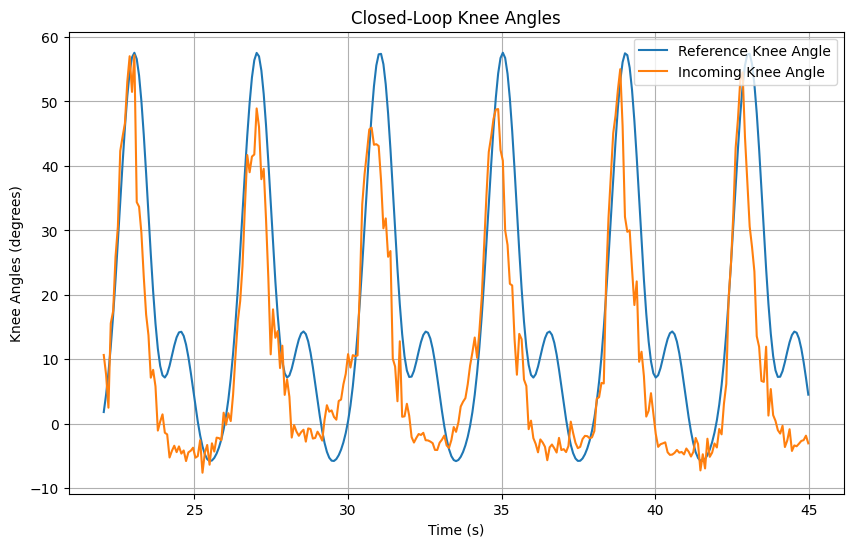
\includegraphics[width=0.95\linewidth]{images/CL9refpng.png}
    \caption{Closed loop knee angles for 0.8km/h}
    \label{fig:cl9ref}
\end{figure}

\begin{figure} [H]
    \centering
    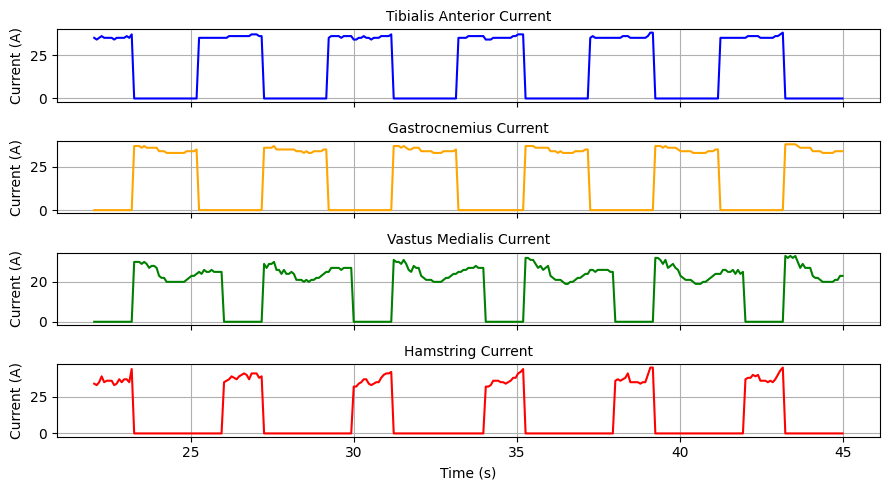
\includegraphics[width=0.9\linewidth]{images/CL9stimpng.png}
    \caption{Closed loop stimulation for 0.8km/h}
    \label{fig:cl9stim}
\end{figure}

Based on the reults seen in figure \ref{fig:cl9ref} and \ref{fig:cl9stim}, the closed loop control system demonstartes a resonable ability to follow the major peaks and valleys of the reference knee angle trajectory at the slower speed of 0.8 km/h. The measured knee angle aligns well with the timing and amplitude of the primary peaks. 

However, the system struggles to replicate the smaller peaks and subtler variations in the reference trajectory. This discrepancy could can be attributed to limitations in the PI controls responsiveness to small variations in reference knee angle and delay in muscle response. This issue might however be possible to mitigate by further tuning of the gains. As can be observed in figure \ref{fig:cl9stim} the variation in stimulation amplitude is not very large, indicating that there is room for increasing the gains and thus the variation in intensity.  

Notably, there is minimal delay observed between the initiation of the initial spike in the reference signal and the corresponding response in the measured knee angle. This highlights the control systems rapid reaction time, which is curcial for maintaining synchrnoization with the reference gait pattern.

\todo{talk more about the stimulation and compare with open loop stimulation}

\subsubsection{Faster Speed}
During the faster speed (1.5km/h) the following parameters were tuned and used on the subject:

\begin{table}[h!]
\centering
\caption{Closed Loop Parameters for 1.5km/h}
\begin{tabular}{|l|c|c|c|c|c|}
\hline
\textbf{Muscle}  & \textbf{Feedforward Current (mA)} & \textbf{Stimulation Limit (mA)} & \textbf{$K_p$} & \textbf{$K_i$} \\ \hline
Tibialis Anterior & 35 & 45 & 0.2 & 0.05 \\ \hline
Vastus Medialis   & 20 & 35 & 0.4 & 0.05 \\ \hline
Gastrocnemius     & 35 & 45 & 0.2 & 0.05 \\ \hline
Hamstring          & 35 & 50 & 0.5 & 0.05 \\ \hline
\end{tabular}
\label{tab:closed_loop_12}
\end{table}

\begin{figure} [H]
    \centering
    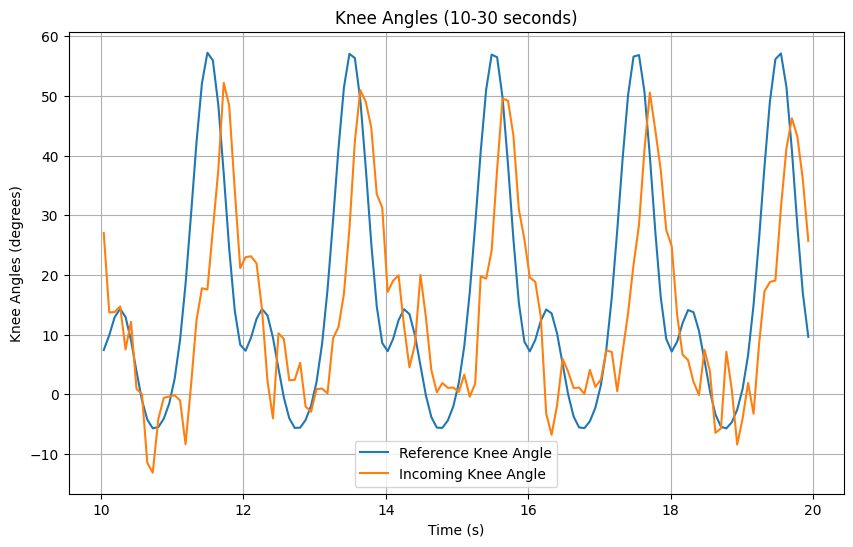
\includegraphics[width=0.9\linewidth]{images/CL12ref.png}
    \caption{Closed loop knee angles for 1.5km/h}
    \label{fig:cl12ref}
\end{figure}

\begin{figure} [H]
    \centering
    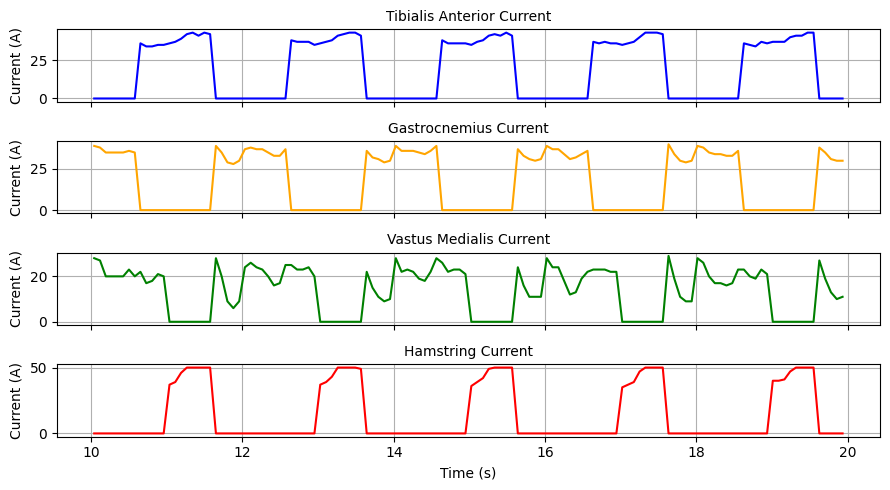
\includegraphics[width=0.9\linewidth]{images/CL12stim.png}
    \caption{Closed loop stimulation}
    \label{fig:cl12stim}
\end{figure}

\todo{Take a look at raw IMU data}
\todo{Take a look at Open loop, compare stim}

At a faster speed of 1.5km/h the results (figure \ref{fig:cl12ref} demonstrate that the closed-loop control system is capable of following the general trajectory of the referance knee angle values. However there is a marked delay between the reference curve and the measured curve, which was not present to the same degree at a slower speed.

Another interesting observation is that the systems seems to more accurately capture the smaller peaks in the trajectory compared to the slower speed. This is likely due to the increased gains in the control system leading to larger variations in the stimulation amplitude as can be seen in figure \ref{fig:cl12stim}.

Compared to the slower speed it is also clear the sampling frequency of the IMU measurements might be becoming an issue at this speed. This is particularly evident during periods of faster transitions, in which the measured signal becomes more jagged and noisy, possibly leading to suboptimal stimulation intensities being applied. 



%=================================================================
%                           End Document
%=================================================================
\end{document}